\chapter{Исследовательская часть}

\section{Интерфейс приложения}

На рисунке~\ref{fig:interface} представлен интерфейс приложения.

\begin{figure}[h!]
	\centering{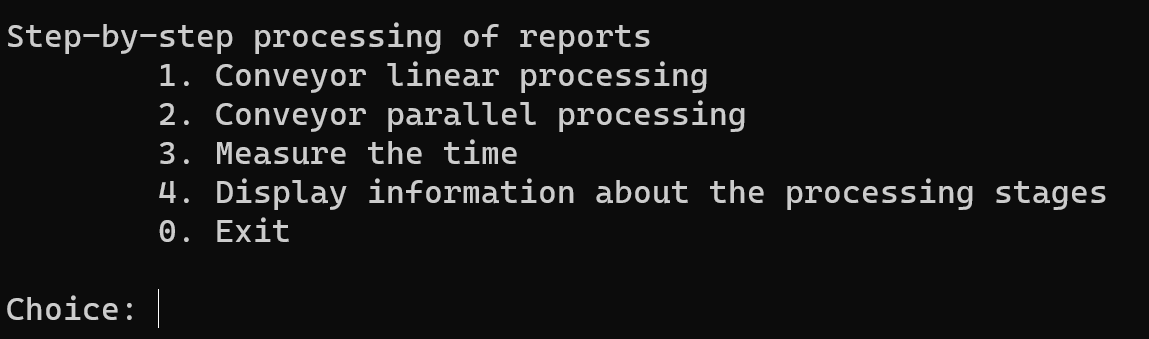
\includegraphics[scale=0.9]{photos/interface.png}}
	\caption{Интерфейс приложения}
	\label{fig:interface}
\end{figure}

\section{Технические характеристики}

Технические характеристики устройства:

\begin{itemize}
	\item операционная система --- Windows 11 Pro 64 -- разрядная система~\cite{windows};
	\item оперативная память --- 16 Гбайт;
	\item процессор --- 11th Gen Intel(R) Core(TM) i7-1165G7 с тактовой частотой 2.8 ГГц.
\end{itemize}

\section{Временные характеристики}

В таблице~\ref{tab01} приведено сравнение времени выполнения параллельной обработки данных в зависимости от количества входных задач.
Линия №1 --- чтение файла, линия №2 --- поиск подстроки в тексте файла алгоритмом Бойера --- Мура, линия №3 --- запись результата в файл.
Время указано в секундах.

\begin{table} [h!]
	\caption{Таблица времени выполнения параллельной обработки данных, время в секундах}
	\label{tab01}
	\begin{tabular}{|r|r|r|r|r|}
		\hline
		К-во задач & Линия №1, с & Линия №2, с & Линия №3, с & Время работы, с\\
		\hline
		50 & 0.03 & 0.16 & 0.01 & 0.27 \\
		\hline
		100 & 0.06 & 0.34 & 0.02 & 0.47 \\
		\hline
		200 & 0.13 & 0.63 & 0.06 & 0.90 \\
		\hline
		400 & 0.30 & 1.32 & 0.15 & 1.86 \\
		\hline
		800 & 0.63  & 2.45 & 0.31 & 3.45 \\
		\hline
	\end{tabular}
\end{table}
\newpage

На рисунке~\ref{fig:linear-vs-parallel} представлен график зависимости времени от количества задач для линейной и параллельной обработки конвейера.

\begin{figure}[h!]
	\centering
	\begin{tikzpicture}
		\begin{axis}[
			ymode = log,
			%	log ticks with fixed point,
			scaled y ticks=real:1e5,
			grid=both,
			xtick={0, 10, 20, 30, 40, 50, 60, 70, 80, 90, 100},
			xticklabel style={/pgf/number format/fixed},
			width=14cm,
			axis lines=left,
			ylabel={Время, мс},
			ylabel style={yshift=10pt},
			xlabel=К-во задач (ед.),
			legend pos=north west,
			]
			\addplot table[x=size,y=Linear,col sep=comma]{graph/linear.csv};
			\addplot table[x=size,y=Parallel,col sep=comma]{graph/parallel.csv};
			\legend{Линейный, Параллельный}
		\end{axis}
	\end{tikzpicture}
	\captionsetup{justification=centering}
	\caption{Зависимость времени работы реализации конвейеров от количества задач}
	\label{fig:linear-vs-parallel}
\end{figure}

%\newpage
\section{Вывод}

В исследовательском разделе были приведены результаты замеров зависимости времени выполнения от количества задач для параллельной и линейной обработки конвейера.

В результате исследования было получено, что параллельная реализация конвейерной обработки данных выполняется быстрее,
чем последовательная приблизительно в 1.1 раза.